\documentclass[cyan]{elegantnote}
\author{Yuyang Songsheng}
\email{songshengyuyang@gmail.com}
\zhtitle{物理}
\entitle{Physics}
\version{1.00}
\myquote{Summary is the best way to say ``Good Bye''}
\logo{logo.jpg}
\cover{cover.pdf}
%green color
   \definecolor{main1}{RGB}{210,168,75}
   \definecolor{seco1}{RGB}{9,80,3}
   \definecolor{thid1}{RGB}{0,175,152}
%cyan color
   \definecolor{main2}{RGB}{239,126,30}
   \definecolor{seco2}{RGB}{0,175,152}
   \definecolor{thid2}{RGB}{236,74,53}
%cyan color
   \definecolor{main3}{RGB}{127,191,51}
   \definecolor{seco3}{RGB}{0,145,215}
   \definecolor{thid3}{RGB}{180,27,131}

\usepackage{mhchem}
\usepackage{makecell}
\usepackage{lipsum}
\usepackage{amssymb}
\usepackage{float}
\usepackage{wrapfig}
\usepackage{latexsym}
\usepackage{hyperref}
\usepackage{feynmf}
\usepackage{exscale}
\usepackage{relsize}
\usepackage{slashed}
\usepackage{mathrsfs}
\usepackage{bm}%bold math, for vector


\begin{document}
\maketitle
\tableofcontents
\chapter{Weak Field Limit}
\section{The linearized theory of gravity}
In a weak-field situation
\[g_{\mu\nu} = \eta_{\mu\nu} + h_{\mu\nu} \quad |h_{\mu\nu}| \ll 1,\]
one can expand the field equations in powers of $h_{\mu\nu}$
using a coordinate frame where $|h_{\mu\nu}| \ll 1$ holds; and without much loss of accuracy, one can keep only linear terms. The resulting formalism is often called ``the linearized theory of gravity''. The resulting connection coefficients, when linearized in the metric perturbation $h_{\mu\nu}$, read 
\[\Gamma^{\mu}_{\alpha \beta} = \frac{1}{2}\eta^{\mu\nu} (h_{\alpha\nu,\beta} + (h_{\beta\nu,\alpha} - h_{\alpha\beta,\nu}) \equiv \frac{1}{2}(h_{\alpha \phantom{*},\beta}^{\phantom{*} \mu} + h_{\beta \phantom{*},\alpha}^{\phantom{*} \mu} + h_{\alpha\beta}^{\phantom{**} ,\mu} )\]
Whenever one expands in powers of $h_{\mu\nu}$, indices of $h_{\mu\nu}$ are raised and lowered using $\eta^{\mu\nu}$ and $\eta_{\mu\nu}$, not $g^{\mu\nu}$ and $g_{\mu\nu}$. A similar linearization of the Ricci tensor yields
\[R_{\mu\nu} = \Gamma^{\alpha}_{\phantom{*}\mu\nu,\alpha} - \Gamma^{\alpha}_{\phantom{*}\mu\alpha,\nu} = \frac{1}{2}(h_{\mu \phantom{*},\nu\alpha}^{\phantom{*} \alpha} + h_{\nu \phantom{*},\mu\alpha}^{\phantom{*} \alpha} - h_{\mu\nu,\alpha}^{\phantom{***}\alpha} - h_{,\mu\nu})\]
where
\[h \equiv \eta_{\mu\nu}h^{\mu\nu}\]
After a further contraction to form $R \equiv g^{\mu\nu}R_{\mu\nu} \approx \eta^{\mu\nu}R_{\mu\nu}$, one finds the Einstein equations read
\[h_{\mu\alpha,\nu}^{\phantom{***}\alpha} + h_{\nu\alpha,\mu}^{\phantom{***}\alpha} - h_{\mu\nu,\alpha}^{\phantom{***}\alpha} - h_{,\mu\nu} - \eta_{\mu\nu}(h^{\alpha\beta}_{\phantom{**},\alpha\beta} - h_{,\alpha}^{\phantom{*}\alpha}) = 16\pi T_{\mu\nu}\]
Define
\[\overline{h}_{\mu\nu} \equiv h_{\mu\nu} - \frac{1}{2}\eta_{\mu\nu}h\]
the linearized field equations become
\[H^{\mu\alpha\nu\beta}_{\phantom{****},\alpha\beta} = 16\pi T_{\mu\nu}\]
where
\[-H^{\mu\alpha\nu\beta} \equiv \overline{h}^{\mu\nu}\eta^{\alpha\beta} + \overline{h}^{\alpha\beta}\eta^{\mu\nu} - \overline{h}^{\alpha\nu}\eta^{\mu\beta} - \overline{h}^{\mu\beta}\eta^{\alpha\nu} \]
\\
Two different types of coordinate transformations connect nearly globally Lorentz systems to each other: global Lorentz transformations, and infinitesimal coordinate
transformations.\\
Global Lorentz Transformations:\\
\[x^{\mu} = \Lambda^{\mu}_{\phantom{*}\alpha'}x^{\alpha'} \quad \Lambda^{\mu}_{\phantom{*}\alpha'} \Lambda^{\nu}_{\phantom{*}\beta'} \eta_{\mu\nu} = \eta_{\alpha'\beta'} \]
We can verify that $h_{\mu\nu}$ and $\bar{h}_{\mu\nu}$
transform like components of a tensor in flat spacetime
\[h_{\alpha'\beta'} = \Lambda^{\mu}_{\phantom{*}\alpha'} \Lambda^{\nu}_{\phantom{*}\beta'} h_{\mu\nu}\]
Infinitesimal Coordinate Transformations:\\
\[x^{\mu'} = x^{\mu} + \xi^{\mu}\]
where $\xi^{\mu}$ are four arbitrary functions small enough to leave $|h_{\mu'\nu'}| \ll 1$. We can verify that the metric perturbation functions in the new $x^{\mu'}$ and old $x^{\mu}$ coordinate systems are related by
\[h_{\mu\nu}^{\mathrm{new}} = h_{\mu\nu}^{\mathrm{old}} - \xi_{\mu,\nu} - \xi_{\nu,\mu}\]
whereas the functional forms of all other scalars, vectors, and tensors which is of order $O(h)$, such as $R_{\mu\nu}$, $T_{\mu\nu}$ and $R$, are unaltered, to within the precision of linearized theory. 
\\
For any physical situation, one can specialize the gauge so that
\[\overline{h}^{\mu\alpha}_{\phantom{**},\alpha} = 0\] 
called Lorentz gauge. The Lorentz gauge is not fixed uniquely. The gauge condition is left unaffected by any gauge transformation for which
\[\Box \xi \equiv \xi^{\alpha,\beta}_{\phantom{**}\beta} = 0\]
The field equations then become
\[\Box h_{\mu\nu} = -16\pi T_{\mu\nu}\]
Once the gauge has been fixed by fiat for a
given system, one can regard $h_{\mu\nu}$ as components of tensors in flat spacetime; and one can regard the field equations and the chosen gauge conditions as geometric, coordinate-independent equations in flat spacetime.
This viewpoint allows one to use curvilinear coordinates, if one wishes. But in doing so, one must everywhere replace
the Lorentz components of the metric $\eta_{\mu\nu}$ by the metric's components $g_{\mu\nu_{\mathrm{flat}}}$ in the flat-spacetime curvilinear coordinate system; and one must replace all ordinary derivatives in the field equations and gauge conditions by covariant derivatives whose connection coefficients come from $g_{\mu\nu_{\mathrm{flat}}}$.

\section{Nearly Newtonian gravitational fields}
The general solution to the linearized field equations in Lorentz gauge lends itself to expression as a retarded integral of the form familiar from electromagnetic theory:
\[\overline{h}_{\mu\nu}(t,\bm{x}) = \int \frac{4T_{\mu\nu}(t-R,\bm{x}')}{R} d^3x' \quad R = |\bm{x}-\bm{x}'|\]
Here focus attention on a nearly Newtonian source: $T_{00} \gg |T_{0i}|$ and $T_{00} \gg |T_{ij}|$, and velocities
slow enough that retardation is negligible. In this case, we have
\[\overline{h}_{00} = -4\Phi \quad \overline{h}_{0i} = \overline{h}_{ij} = 0\]
\[\Phi(t,\bm{x}) = -\int \frac{T_{00}(t,\bm{x}')}{R} d^3x' = \mbox{ Newtonian potential }\]
The corresponding metric is
\[ds^2 = -(1+2\Phi)dt^2 + (1-2\Phi)(dx^2 + dy^2 + dz^2) \approx -(1-\frac{2M}{r})dt^2 + (1+\frac{2M}{r})(dx^2 + dy^2 + dz^2)\]
For a test particle whose velocity $v \ll 1$, the geodesic equation can be written as
\[\frac{d^2 v^i}{dt^2} + \Gamma^{i}_{00} = \frac{d^2 v^i}{dt^2} + \Phi_{,i} = 0\]
So, we reproduce the classical Newtonian gravitation theory.

\section{Gravitational wave}
Let us decompose $h_{\mu\nu}$ as
\[h_{00} = -2A \quad h_{0i} = \partial_i B + \bar{B}_i \quad h_{ij} = 2C\delta_{ij} + 2\partial_i\partial_j E + \partial _i\bar{E}_j + \partial_j\bar{E}_i + \tilde{E}_{ij}\]
with
\[\partial_i \bar{B}_i = 0 \quad \partial_i \bar{E}_i = 0 \quad \partial_i \tilde{E}_{ij} = 0 \quad \tilde{E}^i_i = 0\]
Then we decompose the displacement vector for gauge transformation as
\[\xi^0 = -T \quad \xi^i = -\partial^i L - \bar{L}^i\]
with
\[\partial_i \bar{L}^i = 0\]
Under such coordinate transformation , the metric transform as
\[A \to A + \dot{T} \quad B \to B + \dot{L} - T \quad C \to C \quad E \to E  + L\]
for the scalar modes,
\[\bar{B}_i \to \bar{B}_i + \dot{\bar{L}}_i \quad \bar{E}_i \to \bar{E}_i + \bar{L}_i\]
for the vector modes, and the tensor modes remain unchanged
\[\tilde{E}_{ij} \to \tilde{E}_{ij}\]
The tensor modes are therefore gauge invariant since they do not depend on the choice of the coordinate system. This is not the case for the vector and scalar modes. However, we can define a combination of these modes that are gauge invariant. For the scalar modes, we define
\[\Phi = A + \dot{B} - \ddot{E} \quad \Psi = -C\]
and for the vector modes
\[\bar{\Phi}_i = \dot{\bar{E}}_i - \bar{B}_i\]
We therefore have defined 2 scalar quantities and 1 vector quantity (2 degrees of freedom) which are gauge invariant. All together , we therefore have $6$ degrees of freedom, once the $4$ arbitrary degrees of freedom related to the gauge choice have been absorbed.
\\ \\
For the scalar modes, the Einstein equation $G_{\mu\nu} = 0$ imply that
\[\nabla^2 \Psi = 0 \quad \partial_i \dot{\Psi} =0 \quad \Phi-\Psi = 0\]
The only regular solutions are
\[\Phi = \Psi = 0\]
which means that no scalar mode can propagate.
\\ \\
For the vector modes, we have
\[\nabla^2 \bar{\Phi}_i = 0\]
the only regular solution is $\bar{\Phi}_i = 0$. Just as for scalar modes, no vector modes can propagate.
\\ \\
For tensor modes, we have
\[\Box \tilde{E}_{ij} = 0\]
So, the only perturbations that can propagate in a Minkowski space-time are the gravitational waves and they satisfy
\[\Box \tilde{E}_{ij} = 0 \quad \partial_i \tilde{E}_{ij} = 0 \quad \tilde{E}^i_i = 0\]
The three conditions $\Phi = \Psi = \bar{\Phi}_i = 0$ define a gauge equivalence class. We can choose a gauge in this family by imposing some conditions on the perturbations. For instance, setting $E = B = 0$ and $\bar{E}_i = 0$, we define what is called a transverse and traceless (TT) gauge in which the metric is completely determined. In this case, the only non-vanishing component of $h_{\mu\nu}^{\mathrm{TT}}$ is $\tilde{E}_{ij}$.
\\ \\
Let us consider a plane wave propagating along the axis $z$ in the TT gauge. Since the wave is transverse and traceless, it satisfies $h_{xz}^{\mathrm{TT}} = h_{yz}^{\mathrm{TT}} = h_{zz}^{\mathrm{TT}} = 0$. Therefore, it has only two degrees of freedom (two polarizations) that should satisfy $h_{xx}^{\mathrm{TT}} = - h_{yy}^{\mathrm{TT}}$ ans $h_{xy}^{\mathrm{TT}} = h_{yx}^{\mathrm{TT}}$. We hence can decompose it as following
\[h_{ij}^{\mathrm{TT}} = E_+(t-z)\epsilon^+_{ij} + E_{\times}(t-z)\epsilon^{\times}_{ij}\]
with the two polarization tensors being define by
\[\epsilon^+ \equiv \begin{pmatrix}
1 & 0 & 0\\ 0 & -1 & 0 \\ 0 & 0 & 0
\end{pmatrix} \quad \epsilon_{\times} \equiv \begin{pmatrix}
0 & 1 & 0\\ 1 & 0 & 0 \\ 0 & 0 & 0
\end{pmatrix} \]
The solution of the propagation equation is $E_{+ / \times} = A_{+ / \times}\cos(k(z-t)+ \phi)$.
\\ \\
Consider the geodesic equation of a test particle in the gravitational field of a gravitational wave in the TT gauge. Since to leading order in perturbation we have $\Gamma^i_{00} = 0$, a particle initially at rest will remain at rest.
Of course, this does not mean that nothing happens , but rather that the frame of reference is co moving with the test particle. To see if anything happens , we should look at the relative motion of two neighbouring particles, which can be done using the geodesic deviation equation. The relative acceleration is given by
\[\nabla_{\bm{u}} \nabla_{\bm{u}} \bm{n} = -R(\bm{n},\bm{u})
\bm{u}\]
To leading order in $v$, we have $u^{\mu} = (1,0)$ and $n^{\mu} = (0,n^i)$, $R^0_{i0j} = -\frac{1}{2}\ddot{h}_{ij}^{\mathrm{TT}}$. So that
\[\frac{d^2n^i}{dt^2} = -\frac{1}{2}\ddot{h}_{ij}^{\mathrm{TT}} n^j\]
Following figure illustrates the deformation of a ring of particles under the influence of a gravitational plane wave propagating along the axis $z$ for each polarization.

\begin{figure}[!h]
\centering
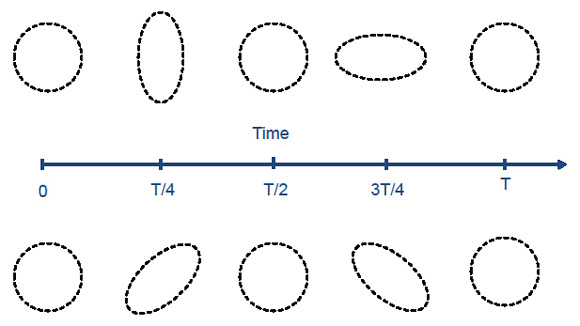
\includegraphics[scale=0.4]{./GR/GW.jpg}
\caption{Effects of a gravitational plane wave propagating along the axis $z$ on a ring of particles located in the plane $xy$, depending on the wave polarization.}
\end{figure}

\chapter{Mass and Angular Momentum of a Gravitating System}
\section{External field of a gravitating source}
Consider an isolated system with gravity so weak that in calculating its structure and motion one can completely ignore self-gravitational effects. Calculate the weak gravitational field
\[\bar{\bar{h}}_{\mu\nu}(t,\bm{x}) \equiv h_{\mu\nu}(t,\bm{x}) = \int \frac{4\bar{T}_{\mu\nu}(t-R,\bm{x}')}{R} d^3x'\]
produced by such a system. Restrict attention to the spacetime region far outside the system, and expand $h_{\mu\nu}$ in powers $\frac{\bm{x}'}{r} \equiv \frac{\bm{x}'}{r}$, we can get
\begin{eqnarray}
ds^2 &=& -\left[1-\frac{2M}{r} + O(\frac{1}{r^3}) \right]dt^2 - \left[4\epsilon_{jkl}S^k \frac{x^l}{r^3} + O(\frac{1}{r^3})  \right] dtdx^i  \nonumber \\
&+& \left[(1+\frac{2M}{r})\delta_{jk} + \mbox{ gravitational radiation terms that die out as } O(\frac{1}{r}) ) \right]dx^j dx^k \nonumber
\end{eqnarray}
where
\[M \equiv \int T^{00}d^3x \quad S_k \equiv \int \epsilon_{klm}x^l T^{m0} d^3x \]
It is plausible to say the mass of the system is $M$ and the angular momentum $\bm{S}$. With an appropriate choice of gauge, $g_{00}$ far from any weak source are time-independent and are determined uniquely by the source's mass $M$; $g_{0j}$ is time-independent and is fixed by the source's intrinsic angular momentum $S^j$; but $g_{jk}$ has time-dependent terms (gravitational waves!) of $O(\frac{1}{r})$.
\\ \\
The values of a system's mass and angular momentum can be measured by probing the imprint they leave in its external gravitational field. 
Of all tools one might use to probe, the simplest is a test particle in a gravitationally bound orbit. 
If the particle is sufficiently far from the source, its motion is affected hardly at all by the source's angular momentum or by the gravitational waves; only the spherical, Newtonian part of the gravitational field has a significant influence. 
Hence, the particle moves in an elliptical Keplerian orbit. To determine the source's mass $M$, one need only apply Kepler's third law
\[M = \left( \frac{2\pi}{\mbox{orbital period}} \right)^2 \left(\mbox{ Semi-major axis of ellipse } \right)^3\]
Angular momentum can be probed by a gyroscope.
Place a gyroscope at rest in the source's gravitational field.
By a force applied to its center of mass, prevent it from falling. 
As time passes, the $g_{0j}$ term in the metric will force the gyroscope to precess relative to the basis vectors $\frac{\partial}{\partial x^j}$; and since these basis vectors are ``tied'' to the coordinate system, which
in turn is tied to the Lorentz frames at infinity, which in turn are tied to the ``fixed stars'' , the precession is relative to the ``fixed stars.'' 
The angular velocity of precession is
\[\bm{\Omega} = \frac{1}{r^3} \left[ -\bm{S} + \frac{3(\bm{S}\cdot \bm{x})\bm{x}}{r^3} \right] \]
One sometimes says that the source's rotation ``drags the inertial frames near the source,'' thereby forcing the gyroscope to precess.
\\ \\
Consider an isolated, gravitating system inside which spacetime may or may not be highly curved. We restrict attention to the weak gravitational field far from the source, and analyze it using linearized theory in vacuum.
Expand $h_{\mu\nu}$ in multipole moments and powers of $\frac{1}{r}$; and adjust the gauge, the Lorentz frame, and the origin of coordinates to simplify the resulting metric.
We have
\begin{eqnarray}
ds^2 &=& -\left[1-\frac{2M}{r} + \frac{2M^2}{r^2} + O(\frac{1}{r^3}) \right]dt^2 - \left[4\epsilon_{jkl}S^k \frac{x^l}{r^3} + O(\frac{1}{r^3})  \right] dtdx^i  \nonumber \\
&+& \left[(1+\frac{2M}{r} + \frac{3M^2}{2r^2})\delta_{jk} + \mbox{ gravitational radiation terms that die out as } O(\frac{1}{r}) ) \right]dx^j dx^k \nonumber
\end{eqnarray}
However, $M$ and $\bm{S}$ is not a simple integration of $T^{00}$ and $\epsilon_{klm} x^l T^{0m}$ of the system as in the case of weakly gravitating sources.
However, since this integration is impossible to measure in practice. We always determine the mass of the star by studying the orbits of planets in its external gravitational field. So, one defines the ``total mass-energy'' $M$ of the sun or other body to be the constant that appears in the line element for its distant external spacetime geometry. Similarly, one defines the body's intrinsic angular momentum as the constant 3-vector $\bm{S}$ appearing in its line element.

\section{Conservation laws for 4-momentum and angular momentum}
Recall in the weak field limit, the Einstein equation can be written as
\[H^{\mu\alpha\nu\beta}_{\phantom{****},\alpha
\beta} = 16\pi T^{\mu\nu}\]
So we have
\[T^{\mu\nu}_{\phantom{**},\nu} = \frac{1}{16\pi}H^{\mu\alpha\nu\beta}_{\phantom{****},\alpha\beta\nu} = 0\]
The source's total 4-momentum can be defined as
\[P^{\mu} \equiv \int T^{\mu 0}d^3x = \frac{1}{16\pi} \oint_{S} H^{\mu\alpha 0 j}_{\phantom{****},\alpha} d^2 S_j \]
Particularly, we have
\[P^0 = \frac{1}{16\pi} \oint_{S} (g_{jk,k} - g_{kk,j})d^2S_{j} \]
The angular momentum of the source can be defined as
\[J^{\mu\nu} \equiv \int (x^{\mu} T^{0\nu} - x^{\nu} T^{0\mu}) d^3x  = \frac{1}{16\pi} \oint_S (x^{\mu}H^{\nu\alpha 0 j}_{\phantom{****},\alpha} - x^{\nu}H^{\mu\alpha 0 j}_{\phantom{****},\alpha} + H^{\mu j 0 \nu} - H^{\nu j 0 \nu}) d^2 S_j \]
\begin{note}
To evaluate the flux integrals (by contrast with the volume
integrals), one need utilize only the gravitational field far outside the source. Since that gravitational field has the same form in full general relativity for strong sources as in linearized theory for weak sources, the flux integrals can be used to calculate $P^{\mu}$ and $J^{\mu\nu}$ for any isolated source whatsoever, weak or strong. So we will use the flux integrals as the definition.
\end{note}

\noindent
Knowing $P^{\mu}$ and $J^{\mu\nu}$, one can calculate the source's total mass-energy $M$ intrinsic angular momentum $S_{rho}$ by
\[M = (-P^{\mu}P_{\mu})^{-1/2}\]
\[Y^{\mu} = -J^{\mu\nu}P_{\nu}/M^2\]
\[S_{\rho} = \frac{1}{2}\epsilon_{\mu\nu\sigma\rho}(J^{\mu\nu} - Y^{\mu}P^{\nu} + Y^{\nu}P^{\mu})P^{\sigma}/M\]
Note especially that the integrands of the flux integrals  are not gauge-invariant. In any local inertial frame at an event they vanish. 
However, the total integrals $P^{\mu}$ and $J^{\mu\nu}$ are. 
They have meaning and significance independent of any coordinate system and gauge. They are tensors in the asymptotically flat region surrounding the source.
\\ \\
In full general relativity, though $|h_{\mu\nu}| \ll 1$ breaks down, we can still define formally
\[-H^{\mu\alpha\nu\beta} \equiv \overline{h}^{\mu\nu}\eta^{\alpha\beta} + \overline{h}^{\alpha\beta}\eta^{\mu\nu} - \overline{h}^{\alpha\nu}\eta^{\mu\beta} - \overline{h}^{\mu\beta}\eta^{\alpha\nu} \quad h_{\mu\nu} \equiv g_{\mu\nu} - \eta_{\mu\nu}\]
And we define the effective energy-momentum pseudotensor by
\[H^{\mu\alpha\nu\beta}_{\phantom{****},\alpha
\beta} = 16\pi T^{\mu\nu}_{\mathrm{eff}}\]
So, we have
\[T^{\mu\nu}_{\mathrm{eff},\nu} = 0\]
\[P^{\mu} = \frac{1}{16\pi} \int d^3x T^{\mu0}_{\mathrm{eff}}\]
\[J^{\mu\nu} = \int (x^{\mu} T^{0\nu}_{\mathrm{eff}} - x^{\nu} T^{0\mu}_{\mathrm{eff}}) d^3x\]
for both strong or weak source.
Define gravitation energy-momentum pseudotensor as
\[16\pi t^{\mu\nu} \equiv H^{\mu\alpha\nu\beta}_{\phantom{****},\alpha
\beta} - 2G^{\mu\nu}\]
so we have
\[T^{\mu\nu}_{\mathrm{eff}} = T^{\mu\nu} + t^{\mu\nu}\]
All the quantities $H^{\alpha\mu\nu\beta}$, $t^{\mu\nu}$ and $T^{\mu\nu}_{\mathrm{eff}}$ depend for their definition and existence on the choice of coordinates.
There is, nevertheless, adequate invariance under general coordinate transformations to give the values $P^{\mu}$ and $J^{\mu\nu}$ of the volume integrals geometric, coordinate-free significance in the asymptotically flat region far outside the source.
Although this invariance is hard to see in the volume integrals themselves, it is clear from the surface-integral forms that no coordinate transformation which changes the coordinates only inside some spatially bounded region can influence the values of the integrals. 
For coordinate changes in the distant, asymptotically
flat regions, linearized theory guarantees that under Lorentz transformations the integrals for $P^{\mu}$ and $J^{\mu\nu}$ will transform like special relativistic tensors, and that under infinitesimal coordinate transformations (gauge changes) they will be invariant.
\\ \\
It is clear that any quantities $H^{\alpha\mu\nu\beta}_{\mathrm{new}}$  which agree with the original $H^{\alpha\mu\nu\beta}$ in the asymptotic weak-field region will give the same values as $H^{\alpha\mu\nu\beta}$ does for the $P^{\mu}$ and $J^{\mu\nu}$ surface integrals. One especially convenient
choice is Landau-Lifshitz pseudotensor. The details can be found in section 96 of \emph{The Classical Theory of Fields (L.D.Landau \& E.M.Lifshitz)}
\\ \\
For a system of gravitating bodies, we have
\[\frac{dP^{\mu}}{dt} = -\oint T^{\mu j}_{\mathrm{eff}}d^2S_j \]
\[\frac{dJ^{\mu\nu}}{dt} = -\oint(x^{\mu}T^{\nu j}_{\mathrm{eff}} - x^{\nu}T^{\mu j}_{\mathrm{eff}}) d^2 S_j\]
The flux is integrated over the surface in asymptomatic flat region. Although the pseudotensor $t^{\mu\nu}$ in the interbody region and outside the system, contributes negligibly to the total 4-momentum and angular momentum, its contribution via gravitational waves to the time derivatives can be important when added up over astronomical periods of time. Thus, one must not ignore it in the flux integrals.
\\ \\
In evaluating these flux integrals, it is especially convenient to use the Landau- Lifshitz form of $T^{\mu\nu}_{\mathrm{eff}}$, since that form contains no second derivatives of the metric. Thus set
\[T^{\mu\nu}_{\mathrm{eff}} = (-g)(T^{\mu\nu} + t^{\mu\nu}_{\mathrm{L-L}}) \approx T^{\mu\nu} + t^{\mu\nu}_{\mathrm{L-L}}\]
Only those portions of $t^{\mu\nu}_{\mathrm{L-L}}$ that die out as $\frac{1}{r^2}$ at large $r$ can contribute to the flux integrals. For static solutions, $t^{\mu\nu}_{\mathrm{L-L}}$ dies out as $\frac{1}{r^4}$. Hence, the only contributions come from dynamic parts of the metric, which, at these large distances, are entirely in the form of gravitational waves. The study of gravitational waves will reveal that when $t^{\mu\nu}_{\mathrm{L-L}}$ is averaged over several wavelengths, it becomes a stress-energy tensor $T^{\mu\nu}_{\mathrm{GW}}$ for the waves, which has all the properties one ever requires of any stress-energy tensor. One can freely make in these integrals the replacement
\[T^{\mu\nu}_{\mathrm{eff}} = T^{\mu\nu} + T^{\mu\nu}_{\mathrm{GW}}\]
So, the rate of loss of 4-momentum and angular momentum from the system, as measured gravitationally, is precisely equal to the rate at which matter, fields, and gravitational waves carry off 4-momentum and angular momentum.

\end{document}